\section{Results}

This chapter presents the results of the classification models that I developed. I focus on comparing the performance of traditional machine learning models, deep learning architectures, and a fine-tuned Large Language Model (DistilBERT) in detecting depression severity across three classes: not depression, moderate, and severe. I evaluated all models using accuracy, F1-score, precision, and recall, with results weighted by class frequencies. Additionally, I also examined confusion matrices to gain insight into class-wise predictions.

\subsection{Machine Learning Models Results}

Table \ref{Table_2} summarizes the performance of traditional machine learning models across two types of feature representations: TF-IDF and sentence embeddings. Among the TF-IDF-based models, the Random Forest classifier achieved the best overall results, with an accuracy of 74.4\% and an F1-score of 74.8\%. It outperformed both Logistic Regression and Linear SVC, which indicates its ability to capture complex feature interactions.

\begin{table}
    \centering
    \caption{Performance of Machine Learning Models}
    \label{Table_2}
    \begin{tabular}{ccccc}
        \toprule
            \textbf{Model}          & 
            \textbf{Accuracy (\%)}  & 
            \textbf{F1 Score (\%)}  & 
            \textbf{Recall (\%)}    & 
            \textbf{Precision (\%)} \\
        \midrule
            Logistic Regression (TF-IDF)      & 67.1 & 65.1 & 67.1 & 68.2 \\
            Linear SVC (TF-IDF)               & 71.8 & 70.7 & 71.8 & 70.9 \\
            Random Forest (TF-IDF)            & 74.4 & 74.8 & 74.4 & 75.4 \\
        \midrule
            Logistic Regression (Embeddings)  & 57.3 & 53.2 & 57.3 & 61.5 \\
            Linear SVC (Embeddings)           & 60.5 & 57.8 & 60.5 & 62.6 \\
            Random Forest (Embeddings)        & 76.3 & 76.4 & 76.3 & 76.6 \\
        \bottomrule
    \end{tabular}
\end{table}

Interestingly, while TF-IDF-based models generally outperformed their embedding-based counterparts, the Random Forest model using sentence embeddings achieved the highest performance across all traditional models, with an accuracy of 76.3\% and an F1-score of 76.4\%. This suggests that Random Forests may be more capable of leveraging the dense semantic information encoded in embeddings compared to linear models.

The confusion matrices for each model, shown in Figure \ref{Fig_2} provide additional insights. The Random Forest (Embeddings) model showed improved classification of the severe class compared to others, which is notable given the severe class imbalance.

\begin{figure}
    \centering
    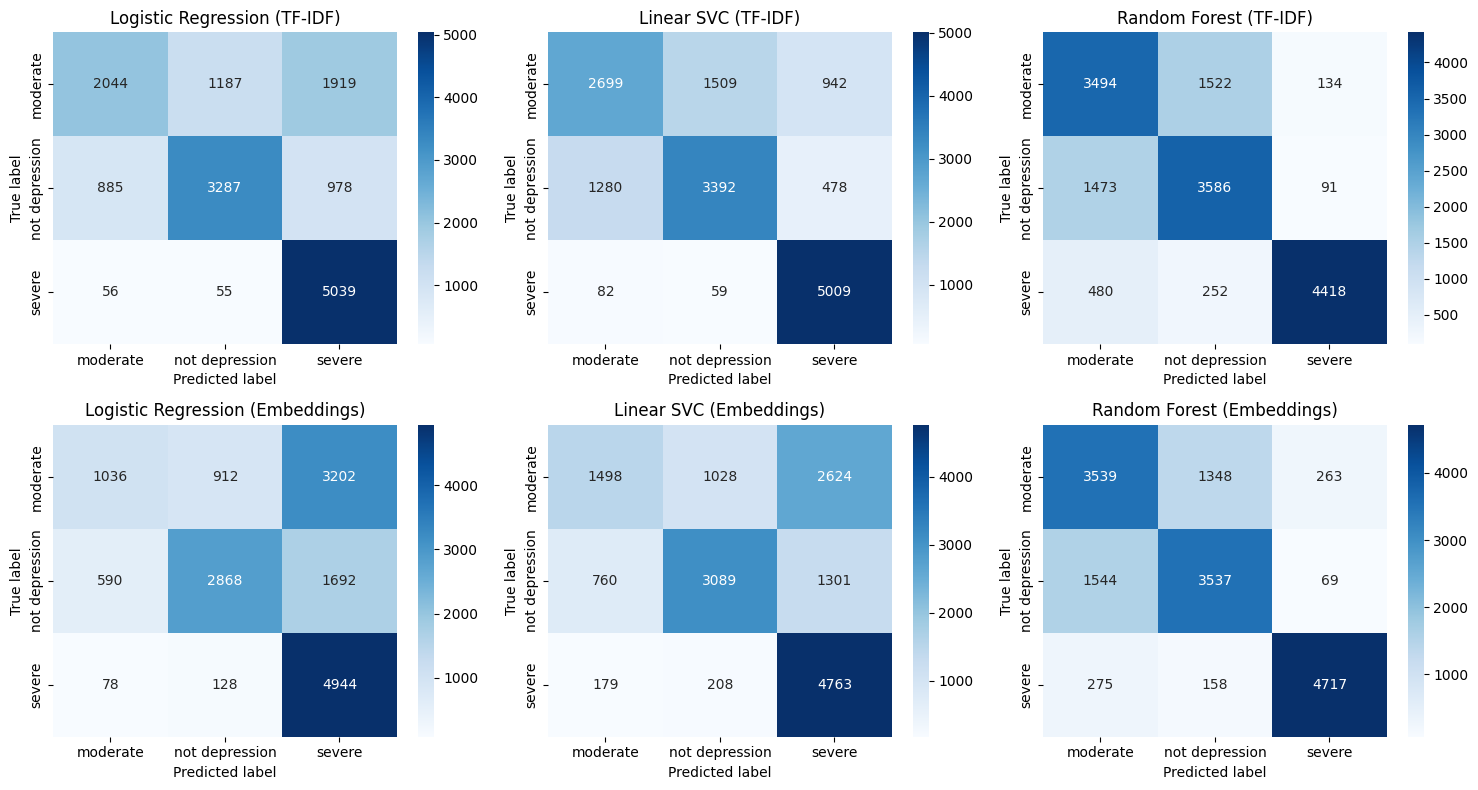
\includegraphics[width=0.8\linewidth]{img/confusion-matrices.png}
    \caption{Confusion Matrices}
    \label{Fig_2}
\end{figure}

\subsection{Deep Learning Models Results}

Table ~\ref{Table_3} displays the results of the BiLSTM models trained with two types of GloVe embeddings: general-domain and Twitter-specific. The BiLSTM model with Twitter-based embeddings slightly outperformed the general GloVe model in F1-score (62.4\% vs. 60.6\%) and precision (64.1\% vs. 62.8\%). This was expected, since domain-specific embeddings should better capture linguistic patterns of social media texts.

\begin{table}
    \centering
    \caption{BiLSTM Models Results}
    \label{Table_3}
    \begin{tabular}{ccccc}
        \toprule
            \textbf{Model}          & 
            \textbf{Accuracy (\%)}  & 
            \textbf{F1 Score (\%)}  & 
            \textbf{Recall (\%)}    & 
            \textbf{Precision (\%)} \\
        \midrule
            BiLSTM (General GloVe)  & 63.3 & 60.6 & 63.3 & 62.8 \\
            BiLSTM (Twitter GloVe)  & 61.4 & 62.4 & 61.4 & 64.1 \\
        \bottomrule
    \end{tabular}
\end{table}

However, both BiLSTM model variants underperformed heavily when compared to the top-performing traditional classifiers. While BiLSTM models may benefit from further hyperparameter tuning or additional data, these results show that their complexity did not translate to superior performance in this setting. I consider that this poor performance is largely due to the limited quality and quantity of the training data, particularly the low representation of severe cases. Moreover, the synonym-replacement data augmentation approach I used may have failed to introduce sufficient new context. For future work, I recommend exploring data augmentation methods based on transformer models like BERT, which can generate more contextually diverse samples.

\subsection{DistilBERT Fine-Tuning Results}

Finally, I evaluated a fine-tuned DistilBERT model using a two-stage training process involving masked language model pre-training followed by supervised classification fine-tuning. The evaluation metrics after 6 epochs are as follows: accuracy of 66.4\%, F1-score of 66.4\%, precision of 66.7\%, and recall of 66.4\%.

While DistilBERT did not outperform the Random Forest classifier with embeddings, it still achieved competitive results and performed better than both BiLSTM models. I attribute its relatively modest performance to similar factors affecting the BiLSTM models: limited quality and quantity of training data and heavy class imbalance. Additionally, unlike with the BiLSTM experiments, no data-level solutions such as augmentation or oversampling were applied here. Given that transformer-based models are more computationally expensive, with sufficient training time and resources, further fine-tuning and extended training could likely improve DistilBERT performance and help it surpass simpler ensemble methods.

In summary, the best performing model across all experiments was the Random Forest classifier trained on sentence embeddings, with an F1-score of 76.4\%. This was followed closely by the TF-IDF version of the same model and the DistilBERT classifier. Deep learning models using BiLSTM performed reasonably but failed to surpass simpler methods.

The confusion matrices reveal that most models struggled with correctly classifying the "severe" class due to its low representation in the dataset. However, augmentation techniques and class weighting helped alleviate this to some extent.